\section{Experiments}\label{sec:exp}

% Table generated by Excel2LaTeX from sheet 'ram config'
\begin{table*}[htbp]
  \centering
  \caption{Device parameters used for I/O buffer, weight buffer and DDR.}
    \begin{tabular}{|r|r|r|r|r|r|r|r|r|}
    \hline
          & bitwidth (B) & size (B) & Rd BW (GB/s) & Wr BW (GB/s) & Rd Ene (pJ) & Wr Ene(pJ) & Leakage (mW) & Area (um\^2)\\
    \hline
    \multicolumn{1}{|c|}{} & 32    & 128K  & 15.169  & 1.556  & 67.690  & 195.286  & 0.04000  & 21224 \\
\cline{2-9}    \multicolumn{1}{|c|}{22nm} & 32    & 256K  & 11.693  & 1.534  & 75.071  & 217.468  & 0.04104  & 26707 \\
\cline{2-9}    \multicolumn{1}{|c|}{LSTP} & 32    & 512K  & 8.005  & 1.490  & 88.483  & 260.073  & 0.04314  & 37308\\
\cline{2-9}    \multicolumn{1}{|c|}{RRAM} & 32    & 1M    & 11.056  & 1.534  & 133.189  & 268.319  & 0.05282  & 61090 \\
\cline{2-9}    \multicolumn{1}{|c|}{} & 32    & 2M    & 10.306  & 1.534  & 231.750  & 357.190  & 0.07806  & 107007 \\
    \hline
    \multicolumn{1}{|c|}{} & 8     & 16K   & 9.145  & 5.147  & 3.057  & 0.556  & 0.00134  & 10031 \\
\cline{2-9}    \multicolumn{1}{|c|}{22nm} & 8     & 32K   & 8.609  & 4.973  & 6.432  & 1.315  & 0.00270  & 20048 \\
\cline{2-9}    \multicolumn{1}{|c|}{LSTP} & 8     & 64K   & 16.831  & 11.763  & 6.780  & 3.777  & 0.00600  & 42803 \\
\cline{2-9}    \multicolumn{1}{|c|}{SRAM} & 8     & 128K  & 10.977  & 10.451  & 7.931  & 2.792  & 0.01153  & 82032 \\
\cline{2-9}    \multicolumn{1}{|c|}{} & 8     & 256K  & 10.977  & 10.451  & 11.562  & 6.424  & 0.02306  & 164065 \\
    \hline
    \multicolumn{1}{|c|}{DDR4} & 4    & 128M  & \multicolumn{2}{c|}{3.2} & 80.300  & 82.719  & 52.80000  & N/A \\
    \hline
    \end{tabular}%
  \label{tab:device}%
\end{table*}%

Experiments are carried out on the architecture introduced in Section~\ref{sec:hw}, with the scheduling strategy in section~\ref{sec:schedule} applied. We use a behavior level simulator to analyze the memory access and computation energy for running a certain network. Memory access dynamic energy cost, memory static energy cost and computation energy cost are considered in our model.

\subsection{Experiment setup}
The MAC array in the architecture is configured as an $8\times8\times8$ array running at 1GHz. This offers a peak performance of 1TOP/s. 8bit multiplication and 32bit accumulation is adopted in this model. Multiplication and addition energy is scaled down from the data in~\cite{mac_energy} to 22nm technology. 

The above configuration requires the read bandwidth of input/output buffer and weight buffer to be at least 64GB/s. We implement each buffer with 8 banks and each of them should offer 8GB/s read bandwidth. On-chip memory parameters are generated from NVSim~\cite{dong2014nvsim} with different memory size configuration. To achieve enough bandwidth, RRAM buffer bit width is configured as 256bit. 

The external memory parameter is generated from MICRON DDR4 power calculator~\cite{powercalc}. The generated dynamic I/O power is further converted to energy per read or write byte. In our experiment, we use 2 DDR chips as external memory because the bandwidth can support the configured MAC array with proposed schedule strategy and the size is enough. In order to reduce background power overhead, we use the least number of chips. All the detailed data and configuration is shown in Table~\ref{tab:device}. 

The buffer in the accumulator is also considered in our experiments. 4 types of buffer is chosen for design space exploration. Corresponding parameters are generated by NVSim and are shown in Table~\ref{tab:small_buf}.

\begin{table}[htbp]
  \centering
  \caption{32-bit accumulation buffer parameters.}
    \begin{tabular}{|r|r|r|r|r|}
    \hline
    depth & 16    & 32    & 64    & 128 \\
    \hline
    energy per read (pJ) & 0.045 & 0.056 & 0.107 & 0.12 \\
    \hline
    energy per write (pJ) & 0.022 & 0.031 & 0.083 & 0.094 \\
    \hline
    \end{tabular}%
  \label{tab:small_buf}%
\end{table}%

\subsection{Design Space Exploration}
We do experiments on all the combinations of the RAM configurations in Table \ref{tab:device} and \ref{tab:small_buf}, which means $5\times 5\times 5 = 125$ choices for a SRAM or RRAM based accelerator. The three schedule strategies in section~\ref{sec:schedule} is applied to each choice. Figure~\ref{fig:design_space} shows the experimental result with the convolution layers of VGG-11 network for 1 input. The energy cost for computation and DDR leakage is marked. These energy cost is the same for all the designs because the network is fixed and all the designs are computation bounded. So the processing time is a constant to all the designs. In general, the RRAM based design consumes less energy compared with an SRAM design of the same area.

\begin{figure*}[t]
  \centering
  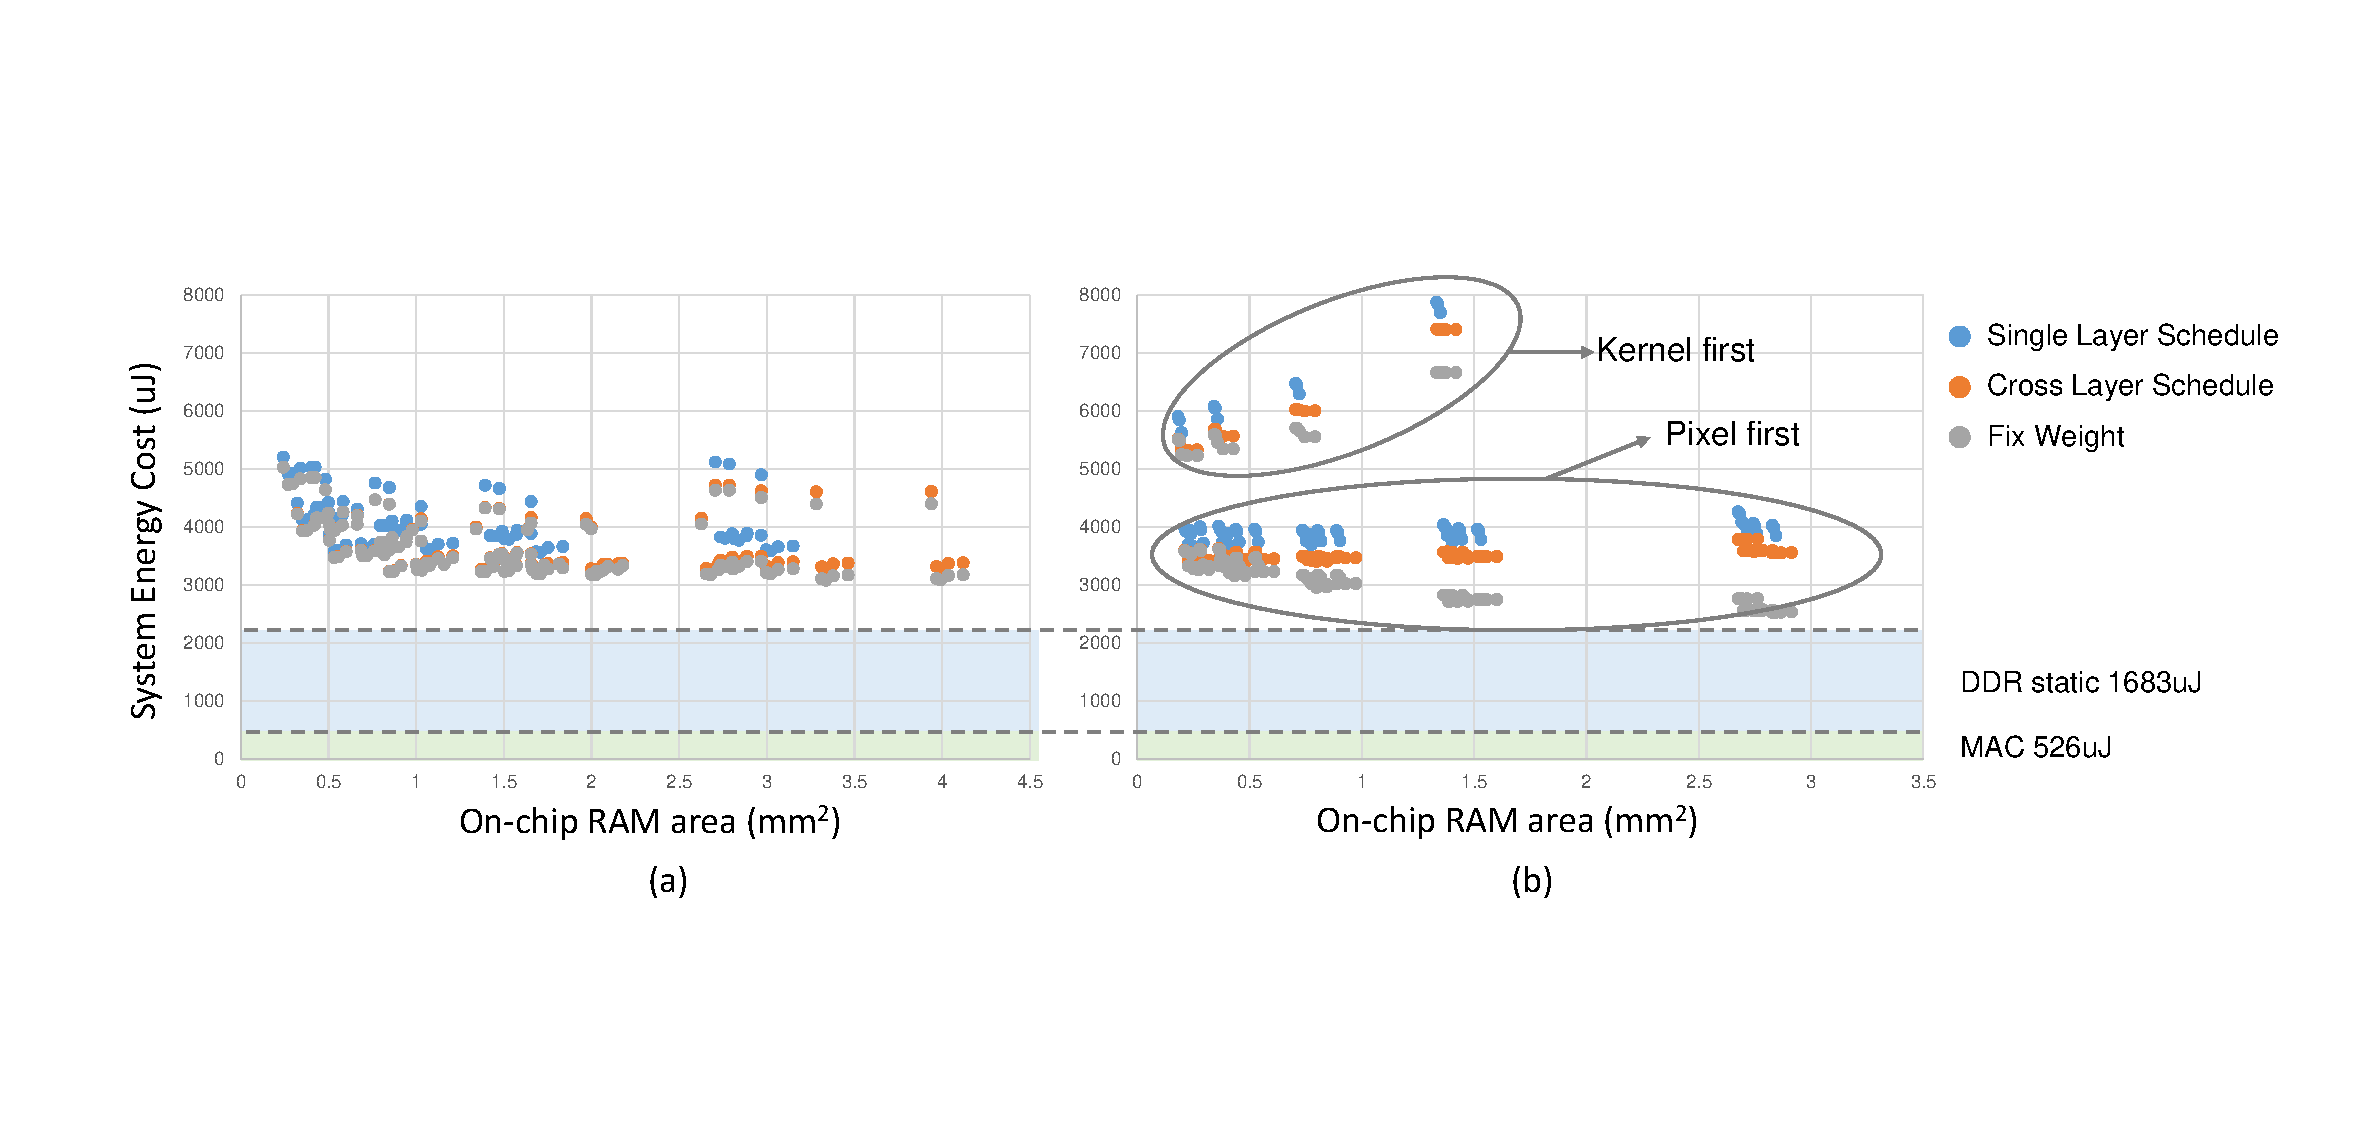
\includegraphics[width=2\columnwidth]{fig/design_space.pdf}
  \caption{Design space exploration on different hardware choices and schedule strategies on the convolution layers of VGG-11 model. (a) SRAM weight buffer design. (b)RRAM weight buffer design.}
  \label{fig:design_space}
\end{figure*}

We examine the effect of the proposed hardware optimization and scheduling strategy. First, the loop order is the key effect to the RRAM based design, as shown in Figure~\ref{fig:design_space}(b). Note that some of the design points with the kernel first loop order are out of the figure because the energy cost is larger than 8000uJ. The large read energy of RRAM dominates the system energy as the capacity of RRAM increases. The reduction in DDR access cannot compensate for this overhead. Even on the smallest design, changing the loop order to pixel first will save at least 1/3 of the system energy cost. 

A breakdown on the on-chip buffer energy cost is shown in Figure~\ref{fig:breakdown}(a). The largest designs, in our experiment the designs with 4MB SRAM input/output buffer and 2MB SRAM (or 16MB RRAM) weight buffer are used. Here we only consider the read energy of input/output buffer and weight buffer and the dynamic energy of accumulation buffer. The write energy to input/output buffer and leakage energy are not affected by the accumulation buffer and thus not considered. Up to $96\%$ energy is saved for the RRAM based designs consider the overhead brough by the accumulation buffer. SRAM design also benefits from the change in loop order but not as effective as to the RRAM designs.

\begin{figure*}[t]
  \centering
  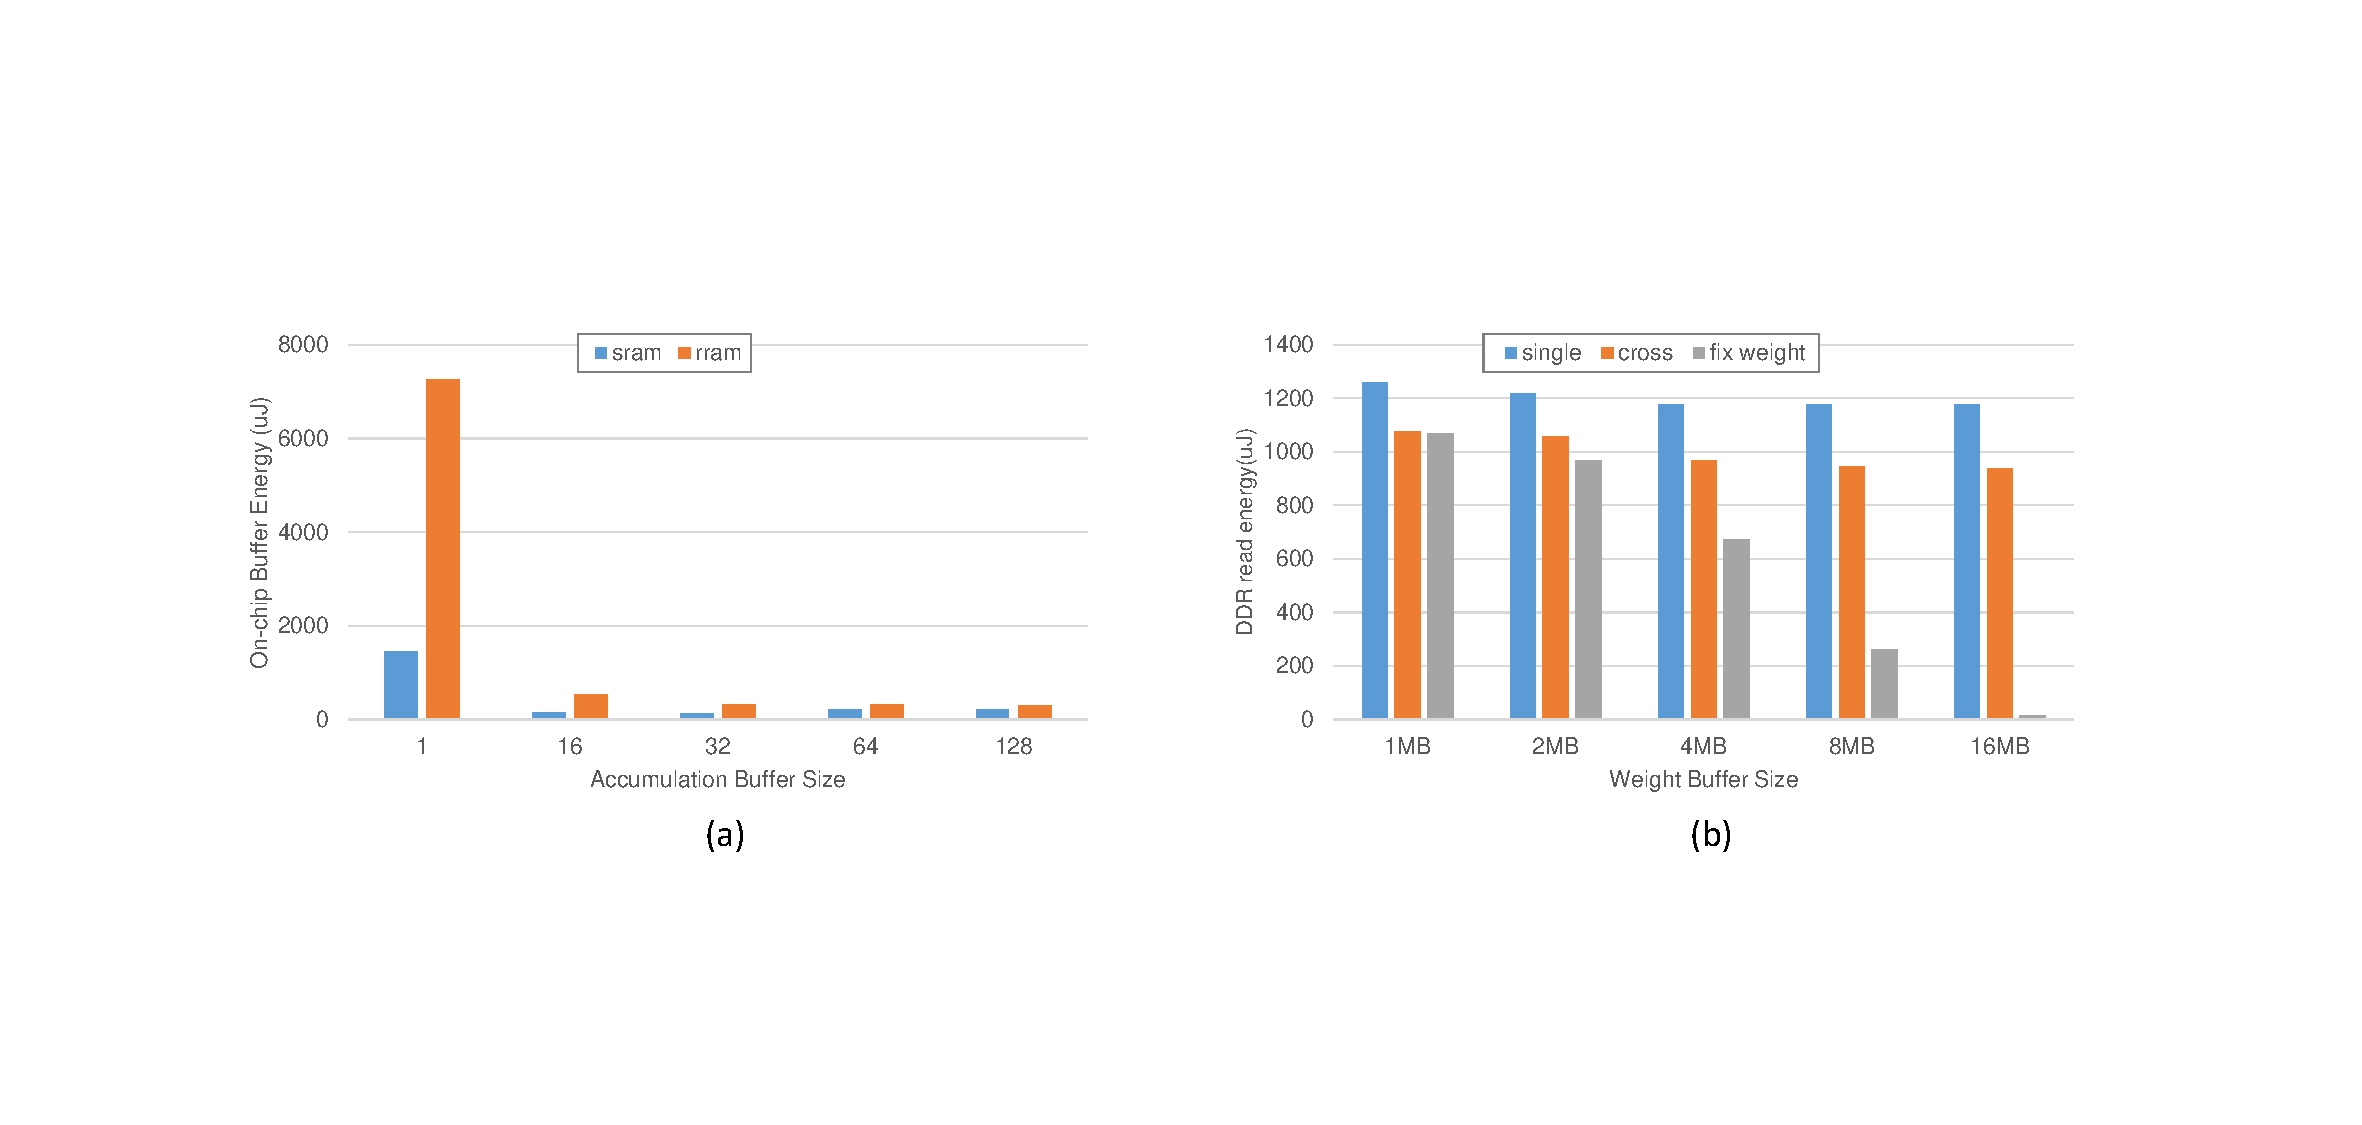
\includegraphics[width=2\columnwidth]{fig/breakdown.pdf}
  \caption{(a) On-chip buffer energy cost for a series of designs only differs in accumulation buffer size. (b) DDR access energy cost for a series of designs only differs in weight buffer size.}
  \label{fig:breakdown}
\end{figure*}

Second, fixing the weight on-chip helps the hardware fully utilize the on-chip RAM to reduce off-chip data transfer. As can be seen from Figure~\ref{fig:design_space}(b), using the pixel first loop order, the accelerator cannot benefit from larger on-chip buffer with single layer scheduling and cross layer scheduling. By fixing some of the network weights on-chip, the system energy cost is gradually reduced as the on-chip RAM size increases. 

A breakdown on the DDR transfer cost is shown in Figure~\ref{fig:breakdown}(b). All the designs implement no accumulation buffer and 1MB SRAM as input/output buffer. The single layer scheduling and cross layer scheduling can only achieve $6.4\%$ and $13.5\%$ energy saving respecitvely when the weight buffer increases from 1MB to 16MB. With the fix weight strategy, the energy saving is $98.5\%$. 

%\subsection{DDR Access energy optimization}

%DDR access behavior is totally decided by schedule strategy. Here we use the convolution layers of VGG-11 to test the effectiveness of the schedule strategy optimization. Figure~\ref{fig:exp_strategy} shows the experimental results. Input/output buffer is 128KB SRAM and weight buffer varies from 1MB to 16MB RRAM in this experiment. Three levels of optimization is compared: only single layer schedule, cross layer schedule, cross layer schedule and consider fixing weight in buffer. When the weight buffer is small, the main energy saving comes from the cross layer schedule. When the buffer gets larger, fixing weight becomes more important. Up to $20\%$ energy saving can be achieved by the our schedule strategy optimization. From Figure~\ref{fig:exp_strategy}(b), we see that strategy optimization reduces the DDR access energy by $25\%\sim 98\%$ under different memory configurations.

%\subsection{On-chip buffer energy optimization}
%From Figure~\ref{fig:exp_strategy}(a), we see that using a larger buffer is not better. This is caused by the increasing buffer I/O energy and leakage power. An example of energy breakdown is shown in Table~\ref{tab:ene_comp}. Both of the design adopts 1MB SRAM I/O buffer. The SRAM weight buffer is 128KB and the RRAM weight buffer is 1MB. Though the RRAM design has less DDR access energy because of a larger weight buffer, the weight buffer read energy is much higher. This shows the necessity of using buffer, rather than a single register, for accumulation. 

% \begin{table}[htbp]
  \centering
  \caption{Example energy breakdown for a pair of SRAM and RRAM design}
    \begin{tabular}{|r|R{1cm}|r|R{1cm}|r|}
    \hline
          & \multicolumn{2}{c|}{RRAM weight buffer} & \multicolumn{2}{c|}{SRAM weight buffer} \\
    \hline
    read iobuf & 0.29  & 0.01\% & 0.29  & 0.01\% \\
    \hline
    read weight & 2119  & 40.50\% & 383   & 10.85\% \\
    \hline
    read ddr & 841   & 16.10\% & 929   & 26.34\% \\
    \hline
    write iobuf & 1.04  & 0.02\% & 1.04  & 0.03\% \\
    \hline
    write weight & 50.4  & 0.96\% & 0.64  & 0.02\% \\
    \hline
    write ddr & 2.08  & 0.04\% & 2.08  & 0.06\% \\
    \hline
    standby & 1691  & 32.33\% & 1686  & 47.79\% \\
    \hline
    calculate & 526   & 10.05\% & 526   & 14.90\% \\
    \hline
    Total & 5230  &       & 3527  &\\
    \hline
    \end{tabular}%
  \label{tab:ene_comp}%
\end{table}%

%We still use the VGG-11 convolution layers to search for an optimal accumulator buffer depth. For each depth choice, we search the optimal buffer size configuration with all the schedule strategy optimization applied. The results are shown in Figure~\ref{fig:exp_buf_depth}. As can be seen from the figure, both methods benefits from the accumulation buffer, but the RRAM design benefits more. With the accumulation buffer, the total on-chip buffer energy cost can be reduced by $86\%$. Combining schedule optimization and accumulation buffer design, we can finally achieve $18\%$ energy reduction by introducing RRAM into on-chip buffer design.